\documentclass[a4paper,12pt]{extarticle}

\usepackage[utf8]{inputenc}
\usepackage[francais]{babel}
\usepackage[T1]{fontenc}
\usepackage[pdftex]{graphicx}
\usepackage{url}
\usepackage{color}
\usepackage{wrapfig}
\usepackage{caption}
\usepackage{multirow}
\usepackage{geometry}
\usepackage{listings}
\usepackage{fancyhdr}
\usepackage{graphicx}
\usepackage{titlesec}
\usepackage{titletoc}
\usepackage{enumerate}
\usepackage{subcaption}

\newlength{\ecartnumero}
\setlength{\parindent}{0cm}
\setlength{\ecartnumero}{3mm}
\setlength{\parskip}{1ex plus 0.5ex minus 0.2ex}

\dottedcontents{section}%
	[\dimexpr 5mm+\ecartnumero]
	{}
	{\dimexpr 15mm+\ecartnumero}
	{3.2mm}

\dottedcontents{subsection}%
	[\dimexpr 15mm+\ecartnumero]
	{}
	{\dimexpr 15mm+\ecartnumero}
	{3.2mm}

\dottedcontents{subsubsection}%
	[\dimexpr 20mm+\ecartnumero]
	{}
	{\dimexpr 15mm+\ecartnumero}
	{3.2mm}

\definecolor{blue}{rgb}{0,0,0.8}
\definecolor{green}{rgb}{0,0.8,0}
\definecolor{red}{rgb}{0.8,0,0}
\definecolor{gray}{rgb}{0.5,0.5,0.5}
\definecolor{black}{rgb}{0,0,0}
\definecolor{maroon}{rgb}{0.5,0,0}

\pagestyle{fancy}
\renewcommand{\sectionmark}[1]{\markboth{#1}{}} % set the \leftmark

\fancyhf{}
\fancyhead[L]{\textbf{\leftmark}}
\fancyfoot[C]{\textbf{page \thepage}}
\fancypagestyle{plain}{
	\fancyhf{},
	\renewcommand{\headrulewidth}{0pt}
}

\lstset
{
	basicstyle=\scriptsize\ttfamily,
	morestring=[s]{"}{"},
	morecomment=[s]{?}{?},
	morecomment=[s]{!--}{--},
	commentstyle=\color{green},
	moredelim=[s][\color{black}]{>}{<},
	moredelim=[s][\color{red}]{\ }{=},
	stringstyle=\color{blue},
	identifierstyle=\color{maroon}
}
  
\newcommand{\hsp}{\hspace{20pt}}
\newcommand{\espace}{\vspace{0.3cm}}
\newcommand{\alinea}{\hspace*{0.4cm}}
\newcommand{\espaceInfo}{\vspace{6cm}}
\newcommand{\marge}{\geometry{vmargin=0.5cm}}
\newcommand{\HRule}{\rule{\linewidth}{0.5mm}}
\renewcommand{\headrulewidth}{1pt}
\renewcommand{\footrulewidth}{1pt}
\renewcommand{\thesection}{\Roman{section}}
\renewcommand{\thesubsection}{\alinea\arabic{subsection}}
\renewcommand{\thesubsubsection}{\alinea\alinea\arabic{subsection}.\arabic{subsubsection}}

%opening

\begin{document}
	\begin{titlepage}
		\begin{sffamily}
		\begin{center}
		% Upper part of the page. The '~' is needed because \\
		% only works if a paragraph has started.
		
		
\includegraphics[scale=0.5]{Img/logo/logo_iutangers}~\\[1.5cm]
		
		\textsc{\LARGE Faculté des sciences d'Angers}\\[1.5cm]
		
		% Gros titre
		\HRule \\[0.4cm]
		{ \huge \bfseries Stage en entreprise}{\bfseries  \\[0.4cm]}
		\HRule \\[1.5cm]
		
		% Image
		\begin{center}
			
\includegraphics[scale=1]{Img/logo/logo_fleurymichon}
		\end{center}
		
		%Sous titre
		\textsc{\LARGE Logiciel de communication entre un système MES et des équipements industriels.}\\[1.5cm] 
		
		% Auteurs et superviseurs
		\begin{minipage}{0.6\textwidth}
			\begin{flushleft} \large
			\begin{center}
				\emph{Professeur référent : }\textsf{M.HAMIEZ} \\
				\emph{Tuteur : }\textsf{M.DESCHAMPS} \\
				\emph{Stagiaire : }\textsf{FRESNEAU Quentin}
			\end{center}
			\end{flushleft}
		\end{minipage}
		
		\vfill
		\HRule\\[1cm]
		% Bas de page
		{\large \today}
		
		\end{center}
		\end{sffamily}
	\end{titlepage}
	\clearpage
	
	\tableofcontents
	
	\clearpage

	\section{Remerciements}
		\paragraph{}

	Je tiens à remercier dans un premier temps, toute l’équipe pédagogique de la faculté des sciences d’Angers et les intervenants professionnels responsables de la formation licence professionnelle Logiciel Libre pour avoir assuré la partie théorique de celle-ci.\\
Je remercie également Monsieur Jean-Philippe Hamiez pour les réponses apportées à mes quelques questions durant la période du stage ainsi que pour son aide à l'élaboration du rapport.\\
Je tiens à remercier tout particulièrement et à témoigner toute ma reconnaissance aux personnes suivantes, pour l’expérience enrichissante et pleine d’intérêt qu’elles m’ont fait vivre durant ces quatre derniers mois de stage au sein de l’entreprise Fleury Michon : \\
Monsieur Deschamps Stéphane, chef de projet informatique, mon tuteur, pour m’avoir intégré rapidement au sein de l’entreprise et m’avoir accordé toute sa confiance ; pour le temps qu’il m’a consacré tout au long de cette période, sachant répondre à toutes mes interrogations ; sans oublier pour sa participation au cheminement de ce rapport.\\
Monsieur Boisseau Jérôme, chef de projet informatique, pour son accueil, ses réponses pour les quelques questions que j’ai pu lui poser durant la période de stage ainsi que pour sa participation au cheminement de ce rapport.\\
Messieurs Guilloteau Kevin, Réau Pierrick, Marais Sébastien et Ribreau Fabien avec qui j’ai travaillé en collaboration pour mettre en place le projet.\\
Enfin, j’aimerais terminer par remercier l’ensemble du personnel informatique du site de Pouzauges et de Chantonnay pour leur accueil sympathique et leur coopération professionnelle tout au long de ces quatre mois.\\

	\clearpage
	
	\section{Introduction}
		\paragraph{}

	Dans le cursus de formation de la licence professionnelle Logiciel Libre, le stage est conçu comme un processus d’immersion réelle à la vie professionnelle dans le domaine de l’informatique. Celui-ci complète les six mois de formation théorique par un stage en entreprise de 18 semaines du 01 avril 2017 au 31 juillet 2017.\\
J’ai donc choisi d’effectuer mon stage au sein du service informatique de l’entreprise Fleury Michon à Pouzauges. Le choix de cette entreprise s’est justifié d’abord par le poste de stagiaire en développement informatique qu’elle proposait afin de réaliser un projet. Ainsi, la méconnaissance du langage de programmation qu’elle utilisait pour cette mission (vb.net\textcolor{red}{*}) m’a poussé à choisir cette entreprise afin de m’autoformer sur cette nouvelle technologie et donc d'enrichir mon expérience. Enfin, le choix de cette entreprise s’est aussi justifié pour des raisons géographiques puisqu’elle se situe à 20 km de mon domicile.\\
Au cours de ce stage, je n’ai pas effectué une seule mission mais un ensemble de tâches ayant attrait à un projet global. Celui-ci contractait différentes compétences que pourrait exiger le métier de développeur informatique ou d’analyste programmeur. En quoi consistent ces missions ? Quelles sont leurs utilités pour l’entreprise ?\\
Ce rapport, après une présentation de l’entreprise et de l’équipe informatique en première partie, explicitera dans la deuxième partie l’analyse du besoin et le but précis du projet tout en les positionnant au cœur du fonctionnement courant de l’entreprise. Puis, en troisième partie, il expliquera les différentes tâches que j’ai effectuées, les problèmes rencontrés ainsi que les solutions trouvées.\\
Enfin, on terminera par la présentation du ressenti sur le stage, les compétences contractées durant celui-ci ainsi que mon projet de fin d’études.\\

\espaceInfo{}
\emph{Tous les mots suivi d'un \textcolor{red}{*} sont spécifiés dans le Glossaire.}

	\clearpage
	
	\section{Présentation de l’entreprise}
	
	\subsection{Historique du groupe}
		\paragraph{}

	L’Histoire de Fleury Michon commence à partir de 1905, Félix Fleury s'associe à Lucien Michon, son beau-frère négociant en viande, tous les deux originaires de Vendée. Ils déposent ensemble les premiers statuts juridiques des établissements Fleury \& Michon. De cet instant à aujourd’hui, le développement de l’entreprise Fleury Michon a traversé différentes périodes.\\
\alinea
	La première période se situe entre 1905 et 1950 et correspond aux fondations du groupe. En effet, elles commencent par l’installation des différents bâtiments (notamment Pouzauges en 1934) mais aussi par la production de produits frais, de plats cuisinés et de produits conservés (par salaison) ainsi que des modifications sur leurs recettes avec une innovation dans la cuisson du jambon en 1954.\\
\alinea
    Puis les années de 1960 à 1970 marquent l’arrivée des produits du groupe sur les grandes surfaces avec différentes gammes de produits de charcuterie frais emballées mais aussi des plats cuisinés frais sous vide. Le groupe Fleury Michon commence en 1987 à montrer leur investissement dans la nutrition avec notamment le développement d’une gamme de produits répondant aux besoins nutritionnels d’un sportif de haut niveau.\\
\alinea
    Viens ensuite la période entre 1990 et 2000 qui est marquée par le développement de la notoriété de la société. En effet, elle commence par le développement de sa production avec l’arrivée du surimi et donc d’un nouveau marché pour l’entreprise. Elle se développe dans le marché du catering aérien (restauration à bord d’un avion) et des plateaux-repas (restauration hors domicile). Elle profite aussi de cette période pour reformuler les procédés de fabrication de tous les produits pour supprimer les additifs et limiter le sel et le gras.
En marge du développement de sa production, elle met aussi l’accent sur la croissance de la marque et de son développement à l'international. Ainsi, elle rachète le concurrent français Olida en 1992, réalise un partenariat avec Beretta (en Italie) pour fonder Piatto Freschi Italia en 2002, et un autre avec Martinez Loriente (en Espagne) pour fonder PLATOS TRADICIONALES en 2005. Elle fait aussi l'acquisition de la société Delta Daily Food au Canada en 2006. Aujourd’hui, le groupe Fleury Michon possède 15 sites de production dont 7 à l'international et avec 8 sites de production en Vendée.\\
\alinea
    Enfin, depuis 2010, c’est surtout l’engagement qui est mis en valeur par le groupe avec la signature de deux chartes d’engagements nutritionnels PNNS (Programme National Nutrition Santé) en 2009 et en 2013 et avec le lancement de la campagne \#VenezVérifier. Cette campagne est créée pour montrer aux consommateurs/blogueurs comment le surimi est produit de la pêche du poisson en Alaska jusqu'à leur préparation en Vendée sur le site de traiteur de la mer (TLM\textcolor{red}{*} à Chantonnay) et montrer la transparence sur leur filière porcine. Enfin, en 2017, Fleury Michone devient le premier industriel à signer la charte nutri-score.\\
L’entreprise Fleury Michon a maintenant un peu plus de 110 ans et a su évoluer au fil du temps afin de rester leader sur leur gamme de produits. Nous allons désormais nous pencher sur le statut juridique et les principaux chiffres de l’entreprise Fleury Michon.

	\subsection{L’entreprise Fleury Michon}
		\paragraph{}
	
	L’entreprise Fleury Michon est une Société Anonyme (SA) à conseil d'administration. Elle est composée de 15 sites de production regroupés dans 8 pays à travers le monde avec au total 3805 collaborateurs (dont plus de 80\% répartis en Vendée). L’ensemble de ces sites propose aujourd’hui un panel complet de produit fabriqué comme des plats cuisinés, du blanc de dinde (ou de poulet), du jambon, des ingrédients pour cuisine, des boxs, des produits tartinables, de la viande à poêler, des viandes rôties et cuisinées, du surimi ainsi que des produits snacking. Elle est d’ailleurs la première marque en part de marché total dans les produits charcuteries, traiteur et traiteur de la mer.\\

\centerline{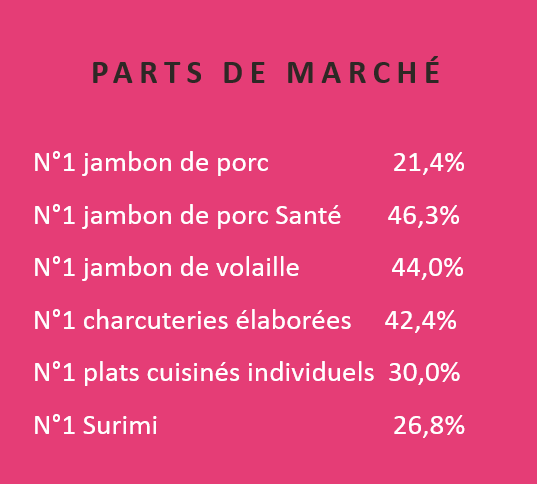
\includegraphics[scale=0.6]{Img/Img_PartMarche.PNG}}
\centerline{\textbf{\underline{Pourcentage des différentes parts de marché.}}}
\espace{}

Elle possède trois pôles d’activité qui sont : 
\begin{enumerate}[-]
	\item le pôle GMS\textcolor{red}{*} libre-service en France (coeur du métier) ;
	\item le pôle international ;
	\item le pôle ventes avec services.
\end{enumerate}

Le pôle GMS, avec 86\% du chiffre d’affaires global, correspond à la distribution en grande surface (hyper/supermarché, proxi, hard/soft discount et e-commerce) dans laquelle les clients visés sont des personnes de tous les jours. Le pôle international est lui aussi concerné par la distribution en grande surface mais aussi par l’export vers d’autres pays. Ce pôle détient 8\% du chiffre d’affaires. Enfin, le troisième pôle correspond aux nouveaux services alimentaires c’est-à-dire le catering aérien (alimentation pour les trajets en avion), le room-saveurs (plateaux-repas ultra frais livrés) et la santé hospitalière (plats cuisinés surgelés). Cette partie de l’activité de l’entreprise détient 8\% du chiffre d’affaires.\\
Le chiffre d’affaires consolidé du groupe Fleury Michon atteint 737,8 millions d’Euros en 2016. Concernant son capital, il est de 13 382 658 Euro. L’entreprise Fleury Michon étant une entreprise familiale et indépendante, on retrouve la répartition du capital comme présentée ci-dessous : \\

\centerline{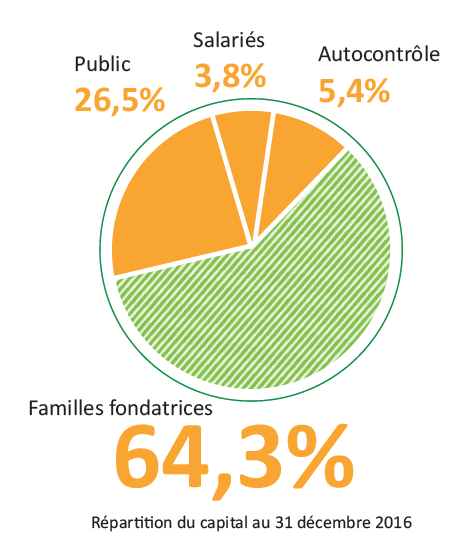
\includegraphics[scale=0.6]{Img/Img_PartCapital.PNG}}
\centerline{\textbf{\underline{Partage du capital du groupe Fleury Michon.}}}
\espace{}

L’entreprise de Pouzauges se divise en différents services : production, maintenance, informatique…(etc). Nous allons désormais nous intéresser davantage au service informatique.

	\subsection{Présentation de l'équipe et des locaux}
		\paragraph{}
	
	Aujourd’hui, le service informatique regroupe une cinquantaine de personnes au sein du DSI (Direction des Systèmes d’Information) dirigé par M. Soulard Gérard et est divisé en 5 pôles majeurs avec : 

\begin{enumerate}[-]
	\item le pôle industriel dirigé par M\up{me} Manceau Marie-Françoise. Ce pôle est chargé de s’occuper de la prévision, la planification, la gestion de production, le système d’exécution de la production (MES) ainsi que la gestion maintenance laboratoire. Ce pôle est divisé en deux équipes, l’une étant disposée sur les différents sites de production et l’autre étant disposé au siège social à Pouzauges ;
	\item le pôle gestion dirigé par M. Gaboriau Vincent. Ce pôle est composé des commerciaux, de la logistique, la FDV (Force De Vente), l’EDI (Échange de Données Informatique), la RH (Ressource Humaine) et la finance ;
	\item le pôle digital dirigé par M. Roux Christophe. Celui-ci est chargé de s’occuper du marketing, de l’Internet et l’Intranet ainsi que des outils de bureautiques et collaboratif (skype, office 365,...) ;
	\item le pôle production informatique dirigé par M. Beucher Stéphane. Ce pôle est responsable de la supervision de la production, des postes de travail, de la téléphonie mobile, ainsi que de l’assistance et des droits ;
	\item et le pôle infrastructure dirigé par M. Babin Laurent. Ce pôle est chargé de s’occuper des systèmes, réseaux et télécoms.
\end{enumerate}

Dans cette organisation, mon responsable de stage M. Deschamps Stéphane est le chef de projet de l’équipe disposé sur site du pôle industriel (voir annexes \emph{Organisation de la DSI}).\\
En revanche, cette organisation a été revue au cours de mon stage avec une fusion des sociétés afin de réorganiser tout le pôle informatique de l’entreprise.\\
Concernant le développement du projet de mon stage, je n’ai pas été amené à travailler avec chacune de ces personnes mais avec certaines d’entre elles, disposé sur différents sites de production.

	\subsection{Situation géographique}
		\paragraph{}

	J’ai passé la plupart du temps de mon stage sur deux sites de production différents. D’abord, sur le site basé à Pouzauges au lieu-dit “La gare” où j’ai réalisé mes premières phases d’analyse et de développement. Ce site est aussi le siège social de l’entreprise. Puis, durant les phases de tests, de modification et d’optimisation, j’ai été amené à travailler sur le site de production de Chantonnay (TLM) qui se situe dans la zone industrielle (Parc Polaris). Ces deux sites sont situés entre 15 et 20 km de mon domicile.\\

\centerline{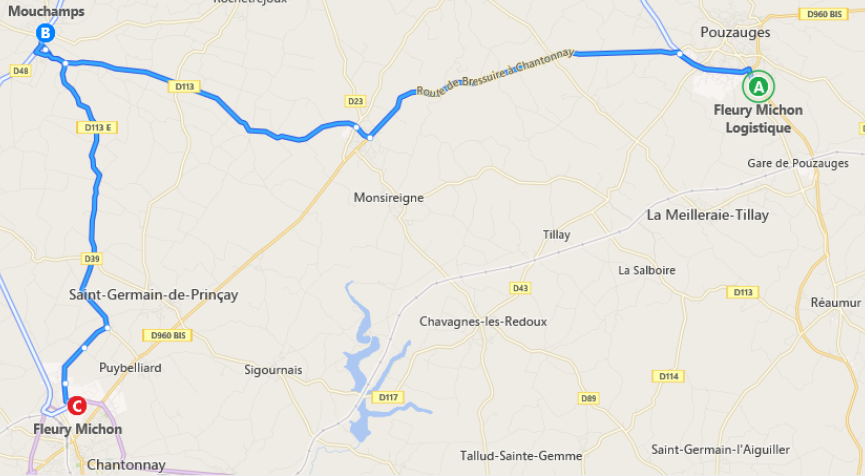
\includegraphics[scale=0.50]{Img/Img_SituationGeo}}
\centerline{\textbf{\underline{Représentation géographique des sites de production TLM et la gare.}}}
\espace{}

	\clearpage
	
	\section{Présentation du projet de stage}
	
	\subsection{Analyse du besoin}
		\paragraph{}
	
	Sur un des sites de production de Chantonnay (TLM) est fabriqué l’un des produits que l’entreprise propose : le surimi.\\
Les dernières étapes du processus de sa fabrication sont le suremballage et la palettisation. Le conducteur de ligne utilise une application de l’entreprise afin d’étiqueter chacun des colis, ceci soit au moment du suremballage ou après la palettisation (selon les lignes de production).\\
Sur une ligne de palettisation, un automate est chargé de communiquer avec deux étiqueteuses de la marque VideoJet afin de pouvoir étiqueter l’ensemble des colis qui composent les palettes arrivant sur le convoyeur.\\

\centerline{\includegraphics[scale=0.5]{Img/Img_SchemaL99.PNG}}
\centerline{\textbf{\underline{Schématisation du principe de fonctionnement de la ligne de production 99.}}}
\espace{}

En revanche, sur une ligne de suremballage, un automate est chargé de communiquer avec une seule étiqueteuse VideoJet qui va alors étiqueter l’ensemble des colis qui arrivent un par un sur le convoyeur. Ce colis, une fois étiqueté est ensuite redirigé en bout de ligne afin de se faire palettiser par un autre employé.\\

\centerline{\includegraphics[scale=0.5]{Img/Img_SchemaL98.PNG}}
\centerline{\textbf{\underline{Schématisation du principe de fonctionnement de la ligne de production 98.}}}
\espace{}

\alinea
	Dans les deux cas, l’application lancée par le conducteur est la même. Celle-ci est nommée MesToColis, elle est chargée de communiquer les informations nécessaires à l’étiquetage tel que la DLC du produit, le numéro de lot, le libellé du produit…(etc) vers les étiqueteuses. Le système existant proposait à l’utilisateur un seul choix d’envoi des données, l’entreprise avait décidé de sous-traiter cet envoi via un petit applicatif nommé iDaro qui scrutait un dossier lors de l’envoi des données. Ce dossier devait alors contenir un masque d’étiquette qui comprenait les informations nécessaires à l’étiquetage. L’application MesToColis venait au préalable charger un masque d'étiquette, modifier le nom des différentes informations par la valeur qui correspondait pour l’OF\textcolor{red}{*} ou l’UT\textcolor{red}{*} sélectionné et sauvegarder le fichier dans le répertoire scruté par l'applicatif. Ce fichier était ensuite lu par le logiciel iDaro qui communiquait ensuite les données vers les étiqueteuses et l’automate.\\

\centerline{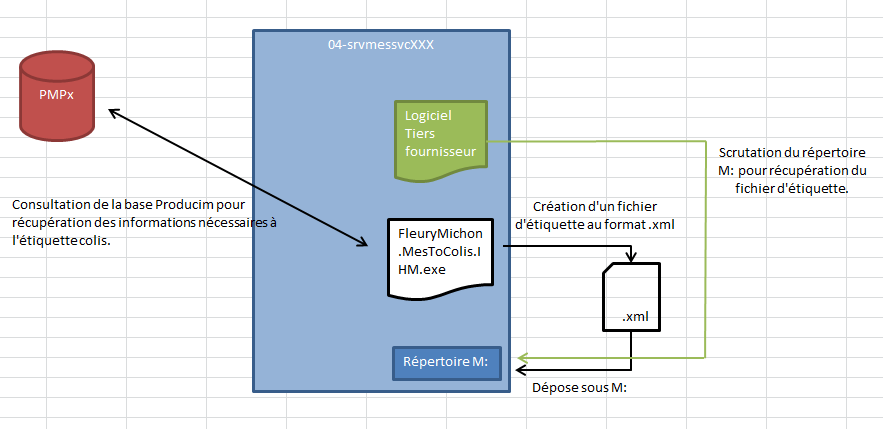
\includegraphics[scale=0.7]{Img/Img_RepresentationiDaro.PNG}}
\centerline{\textbf{\underline{Représentation de l’ancien fonctionnement de l’application.}}}
\espace{}

Ce système fonctionnant sur la ligne 98 du site de production, l’entreprise a souhaité l’implanter sur la ligne 99 mais un problème de réinstallation faisait son apparition. En effet, pour répondre au besoin de l'entreprise, il n'y avait pas d'autre choix que de réinstaller l'applicatif sur un autre serveur de production puisque l'applicatif ne pouvait pas gérer plusieurs connexions. Suite à ça, une autre étiqueteuse a fait son entrée sur la ligne 99 (appelée “Mulet”) qui était utilisé uniquement lorsqu’une des deux étiqueteuses n’avait pas correctement étiqueté certains cartons.\\
Au bout de quelques années, l’entreprise qui sous-traitait cet échange de données n’était plus joignable et pour des raisons évidentes de sécurité et d’indépendance, Fleury Michon a choisi de redévelopper cet échange de données au sein de l’application existante. À la suite d’une réunion, rassemblant les utilisateurs clés et les différentes personnes concernées par le projet lors de la première semaine de mon stage, le but précis du projet, les contraintes ainsi que les délais ont pu être fixés.

	\subsection{But du projet}
		\paragraph{}

	Le but du projet est donc de supprimer le logiciel iDaro. Pour cela, l’entreprise propose de développer en interne à l’application MesToColis l’échange de données vers soit un automate (ou plusieurs) soit une étiqueteuse (ou plusieurs). L’échange entre le MES et une étiqueteuse a été géré au début du mois de février 2017 sur le site de production de Montifaut (MTT\textcolor{red}{*}) par M. Pierrick Réau avec l’utilisation du protocole Zipher Text (transmis par le fournisseur des étiqueteuses VideoJet), il est donc réutilisable à l’avenir.\\
	Sur la ligne 99 de TLM, deux étiqueteuses VideoJet ainsi qu’une troisième nommée Mulet sont gérées par un seul automate de la marque Schneider Electronic. Celui-ci est chargé de communiquer les informations présentes dans le masque d’étiquette ainsi que les informations reçues par l’automate de palettisation aux deux étiqueteuses pour qu’elles puissent étiqueter convenablement les cartons de la palette qui arrive sur le convoyeur. Les informations sont de deux types, celles qui concernent le produit comme par exemple la DLC (Date Limite de Consommation), le libellé et le code du produit… (etc) et celles qui concernent le portique d'étiquetage de la palette c’est-à-dire tous les paramètres que les étiqueteuses doivent prendre en compte pour mener à bien l’étiquetage des colis comme par exemple le nombre de couches de cartons sur la palette, le nombre total de cartons à étiqueter... (etc).\\
	Sur la ligne 98, une seule étiqueteuse VideoJet est gérée par un automate de la même marque. Celui-ci, comme sur la ligne 99, est chargé de communiquer les informations utiles à l’étiquetage. En revanche, il ne reçoit pas d’informations pour le portique d'étiquetage de la palette puisque l’étiquetage se fait directement lorsque le carton arrive devant l’étiqueteuse.\\
\alinea
Pour ce qui est du projet, seule la communication avec le Mulet sur la ligne 99 est souhaitée pour le moment puisqu’elle serait utilisée par les pilotes de ligne en cas de mauvais étiquetage de certains colis de la palette qui arrive sur le convoyeur. Afin de ne pas avoir d’incidence sur la production (en cas de dysfonctionnement), la nouvelle version de l’application MesToColis sera installée dans un dossier différent pour que celle qui fonctionne avec le service iDaro puisse être encore utilisé pour les deux étiqueteuses présentes sur le portique. Ensuite, une fois que la communication entre le MES et l’automate puis de l’automate vers le Mulet sera opérationnelle, l’entreprise pourra basculer ce système pour toutes les étiqueteuses (sur les deux lignes de production concernées) lors d’un arrêt usine.\\

\centerline{\includegraphics[scale=0.9]{Img/Img_ObjectifProjet.PNG}}
\centerline{\textbf{\underline{Schéma de l’objectif du projet.}}}
\espace{}

	\clearpage
	
	\section{Analyse de l'existant}
	
	\subsection{Fonctionnement de l'application}
		\paragraph{}
	
	Voici donc aujourd’hui comment l’application MesToColis se présente : \\

\begin{figure}[h]

\begin{subfigure}{0.5\textwidth}
	\includegraphics[width=0.95\linewidth, height=6cm]{Img/Capture_MesToColisUT.PNG}
	\caption{Mode UT}
	\label{subim1}
\end{subfigure}
\begin{subfigure}{0.5\textwidth}
	\includegraphics[width=0.95\linewidth, height=6cm]{Img/Capture_MesToColisOF.PNG}
	\caption{Mode OF}
	\label{subim2}
\end{subfigure}

	\espace{}
	\centerline{\textbf{\underline{Modes de fonctionnement de MesToColis.}}}
\end{figure}

Tout d’abord, il faut savoir que l'application a deux modes de fonctionnement : le mode OF et le mode UT. Il faut donc commencer par faire la différence entre ce qu’est un OF et une UT. Un OF est un ordre de fabrication pour un produit donné et celui-ci est composé d’UT c’est-à-dire d’unité de traçabilité.\\
Au lancement de MesToColis, 3 paramètres sont obligatoires : le code machine (code 800000), le mode de fonctionnement (1 ou 0) et un entier (0, 1 ou 2) qui représente le droit de modifier les données chargées.\\

\centerline{\includegraphics[scale=0.8]{Img/Capture_ParamApp.PNG}}
\centerline{\textbf{\underline{Capture des paramètres de lancement de l’application.}}}
\espace{}

D'abord, il y a le code machine, il permet de charger les OFs qui sont disponibles sur la machine spécifiée.\\
Ensuite, il y a le mode de fonctionnement, il est soit lancé à 1 (= mode OF) avec un plan de production affichant tous les OFs en cours sur la ligne de production où l’on se trouve. Ou bien, l’application est lancée avec le paramètre à 0 (= mode UT) avec un champ de validation d’UT qui va charger les informations pour une UT rentrée par l’utilisateur.\\
Enfin, le dernier paramètre donne accès à la modification des valeurs chargées lorsqu’il est à 1, des valeurs chargées et des libellés du masque lorsqu’il est à 2 et à aucune modification lorsqu’il est à 0. Concernant le fonctionnement de l’application, ce paramètre reste à 1 afin de pouvoir rentrer le lot UVC qui est une donnée qui n’est pas chargée sur TLM (dans le cas où on est en mode OF).\\
À côté de ces trois paramètres au lancement de l’application, on en retrouve d’autres qui sont internes à l’application. Ceux-là sont compris dans le fichier app.config. Dans celui-ci, on retrouve l’intégralité des paramètres utiles à l’application (le chemin d’accès du masque, du dossier de dépose, de retour et de log, les connexions aux bases de données, les paramètres des étiqueteuses et automates (etc)…).\\
Dans le cadre du projet, on se concentrera sur le paramètre du type de transfert des données qui permet à l’application de savoir quel envoi elle doit réaliser. En effet, ce type/mode de transfert est compris dans la variable “TypeTransfert” et possède aujourd’hui trois valeurs possibles schématisées ci-dessous.\\

\centerline{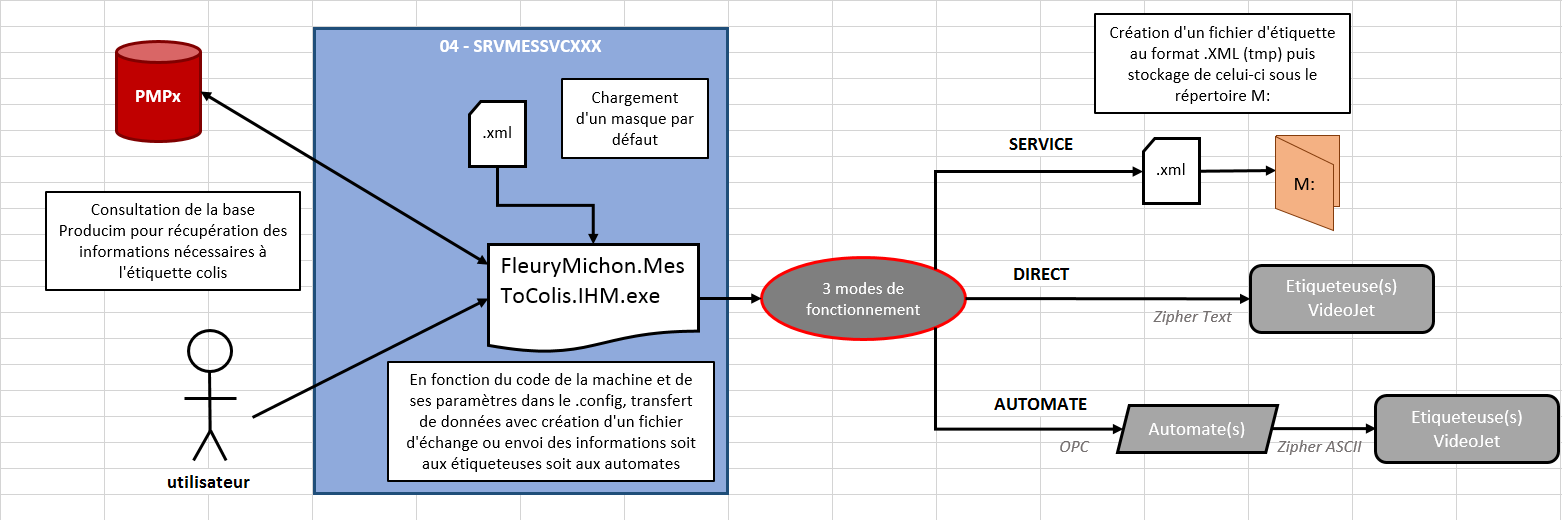
\includegraphics[scale=0.45]{Img/Img_RepresentationProjet.PNG}}
\centerline{\textbf{\underline{Représentation du nouveau fonctionnement de l’application.}}}
\espace{}

D’abord il y a le mode “DIRECT”. Celui-ci, va lire les paramètres des étiqueteuses et va directement générer un message comprenant les informations à étiqueter qui sera interprété par les étiqueteuses pour qu’elles puissent étiqueter les informations à imprimer.\\
Aussi, on retrouve le mode “SERVICE”. Celui-là, va copier le fichier de masque et modifier le code de chaque information par sa valeur. L’application va ensuite sauvegarder ce fichier sur le dossier qui est inscrit dans les paramètres de l’application. Une fois réalisé, le service iDaro vient scruter ce dossier afin de traiter les données du fichier pour ensuite les distribuer vers les étiqueteuses et l'automate. Cette solution a été adoptée par l’entreprise puisqu’elle a été proposée par le fournisseur des étiqueteuses VideoJet.\\
Enfin, on a le nouveau mode “AUTOMATE”. C’était le but du projet : pouvoir directement communiquer les informations utiles à l’étiquetage vers un automate. Dans ce mode, lors de l’envoi des données, l’application vient initialiser une communication avec l’automate (préconfiguré dans le fichier de configuration) puis envoyer les informations chargées.\\
Dans les trois cas, la finalité est la même, l’étiqueteuse VideoJet sort une étiquette (pensé par l’entreprise) directement collée sur le colis (sauf pour le Mulet).

	\subsection{Structure des étiquettes colis}
		\paragraph{}

	Au lancement de l’application MesToColis, un masque d’étiquette (fichier informatique) doit être chargé pour pouvoir afficher les informations nécessaires à l’étiquetage. Ainsi, on retrouve deux types d’informations au sein d’un masque : le libellé et sa valeur. Ces deux informations sont identifiées dans une base de données et viennent structurer l’étiquette souhaitée.\\

\emph{\underline{Exemple :}}\\
	L'information “CODE\_PRODUIT” présente sur le masque va afficher sur l’application le libellé : “Code Produit”.\\
	Le code “CODE\_PROD” va chercher la valeur du code produit dans une base de données (ex : 008456).\\

\emph{\underline{Autre exemple plus spécifique :}}\\
	L'information “LOT” présente sur le masque va afficher sur l’application le libellé : “Lot UVC”.\\
	Le code “GP10057” va chercher la valeur du lot UVC dans une base de données (ex : F8171040).\\

Au fil du temps, des changements sur la structure de l’étiquette ont été réalisés. En effet, avec le choix du fournisseur VideoJet pour les étiqueteuses, l’entreprise avait proposé une première étiquette sur laquelle il y avait un code à barres pour le portique de TLM (en bas), un autre pour la logistique (en haut à gauche) ainsi qu’un QR Code (en haut à droite) disposé comme ci-dessous : \\

\centerline{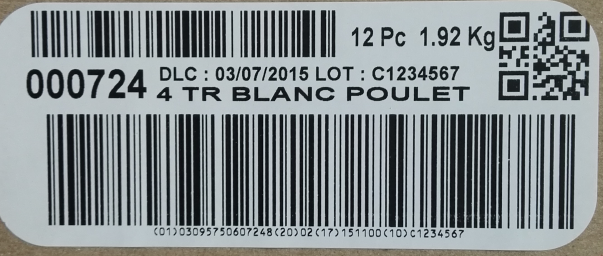
\includegraphics[scale=0.6]{Img/Img_EtiqVJAvant.PNG}}
\centerline{\textbf{\underline{Exemple d’une ancienne étiquette.}}}
\espace{}

Cependant, à cause d’un problème de relecture du code à barres de l’étiquette par le fournisseur (conflit entre les deux codes à barre et le QR Code), un changement a été réalisé sur celle-ci.\\
Aujourd’hui, l’étiquette est disposée comme ceci : \\

\centerline{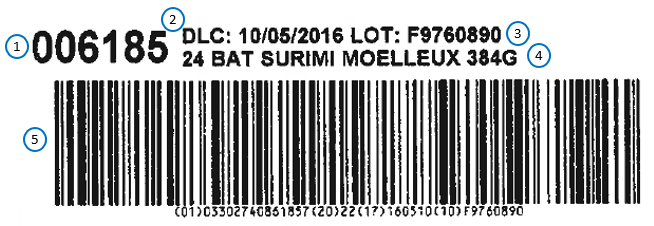
\includegraphics[scale=0.6]{Img/Img_EtiqVJApres.PNG}}
\centerline{\textbf{\underline{Exemple d’une étiquette actuelle.}}}
\espace{}

Sur cette étiquette, on peut y apercevoir les mêmes informations mises à part le PCB (Par Combien) et le Poids (*) puisque ces informations ne sont plus utilisées aujourd’hui.\\
On retrouve donc les informations suivantes : \\
1 - le code produit (code à 6 chiffres) ;\\
2 - la DLC soit au format jj/mm/aaaa (format standard) soit au format aa/qqq (année sur 2 caractères et quantième sur 3 caractères) ;\\
3 - le lot UVC du produit ;\\
4 - le libellé du produit ;\\
5 - un code-barre contenant le GTIN (Global Trade Item Number), la VA, la DLC et le lot UVC du produit.\\

	\clearpage

	\section{Élaboration du projet}
	
	\subsection{Partage du travail}
		\paragraph{}

	Étant en entreprise, le travail effectué au niveau du développement n’a pas été partagé puisque le projet m’était destiné. En revanche, j’ai travaillé avec plusieurs personnes pour pouvoir avancer dans le projet lorsque j’étais face à des difficultés ou par pure prise d’information.\\
J’ai donc travaillé en collaboration avec Deschamps Stéphane, Guilloteau Kevin, Réau Pierrick, Marais Sébastien, Clairet Arnaud, Ribreau Fabien et Bibard Nicolas pour lancer et mener à bien ce projet.\\
Dans le cadre du nouveau fonctionnement de l’application MesToColis pour le site TLM, à Chantonnay, je me suis occupé de la moitié de la communication des données entre le logiciel MES et l’automate et M. Marais Sébastien s’est occupé de l’autre moitié de la communication entre l’automate et les étiqueteuses.

	\subsection{Serveurs et matériel mis à disposition}
		\paragraph{}
			
	Lors de mon arrivée en entreprise, un ordinateur ThinkPad (intel inside, Core i5, 4Go de RAM) m’a été distribué. C’est avec celui-ci que j’ai réalisé toutes les tâches rencontrées au cours de la période du stage. Enfin, pour les phases de tests et de débogage de l’application, M. Marais Sébastien m’a mis en place un automate Schneider M340 muni d’un afficheur tactile pour pouvoir observer le comportement de l'envoi de données par le logiciel MES et pour avoir un visuel sur la validité des valeurs réceptionnées dans les différents espaces mémoires de l'automate. Enfin, pour la dernière phase de test d'étiquetage, l’étiqueteuse VideoJet (nommé Mulet) de référence 9550 a été installé dans le bureau de Sébastien Marais afin de pouvoir tester l’impression des étiquettes.\\
\alinea
	Concernant les serveurs de l’entreprise, chaque site de production possède un lien vers les serveurs du siège social mais des serveurs tampon ont été prévu sur chaque site pour pallier à une éventuelle coupure de réseau. On va maintenant se pencher sur les serveurs qui sont utilisés par le MES. Ceux-là sont gérés avec Windows 2008 R2 x64 Std, on décompte 5 types de serveurs pour la plateforme MES (voir annexes \emph{Architecture des serveurs MES}) : 

\begin{enumerate}[-]
	\item le serveur de base de données nommée 01 - SRVMESBDDxxx (xxx correspondant aux lettres du site) qui contient une base de données (Oracle Server 11gr2 x64) nommée PMPx (x pour le numéro du site correspondant) ;
	\item les serveurs d’applications nommées 02 - SRVMESTSExxx et 03- SRVMESTSExxx, c’est sur ces serveurs-là que sont installées les différentes applications. Dans le cadre du site de production de TLM, il y a 4 TSE (02, 03, 06 et 07) sur lesquelles on retrouve une installation de MesToColis ;
	\item le serveur de services et d’interfaces nommées 04- SRVMESSVCxxx. Dans celui-ci, on y retrouve tous les services et interfaces utilisés en production pour les différentes applications. On y retrouve aussi une base de données d’acquisition nommée ACPx qui regroupe l’ensemble des informations sur les automates... (etc).
Enfin, on retrouve sur ce même serveur le lecteur M: qui permet la communication de documents vers le serveur de la gare (siège social) ;
	\item le serveur de test nommé 90- SRVMESTSTxxx qui contient le contenu des trois serveurs précédents ;
	\item et le serveur de sauvegarde nommée 05- SRVMESSAUxxx.
\end{enumerate}

Durant mon stage, j’ai utilisé ces différents serveurs pour réaliser les installations sur les serveurs de production et le serveur de test de TLM. Pour ce qui est du développement de l’application, j’ai utilisé le logiciel Visual Studio. L'application MesToColis était disponible sur le dossier Référentiel du serveur de développement de la gare (450-SRVDEVGARE ou 94-SRVMESACQDEV).
	
	\subsection{Réalisation hors rapport}
		\paragraph{}
	
	En marge de ce rapport, il a aussi fallu rédiger quelques documents nécessaires à la compréhension des modifications réalisées sur l’application mais aussi à l’explication de son fonctionnement. J’ai donc rédigé un mode opératoire pour les personnes qui utilisaient l’application ainsi qu’une spécification détaillée sur le nouveau fonctionnement de celle-ci pour que le code existant puisse être repris et compris par une autre personne de l’entreprise. Cette spécification détaillée a donc été ajoutée au sein de l’intranet de l’entreprise.\\
Aussi, pour faciliter la rédaction du rapport de stage, j’ai utilisé Google Drive et mis en place un GIT (voir lien dans sources) dans lequel je m’étais à jour chaque semaine un journal de bord et un descriptif des problèmes rencontrés (et de leurs solutions) pendant toute la période du stage mais aussi pour y stocker les différents fichiers utiles à l’élaboration du rapport. J’y ai aussi ajouté un diagramme de Gantt dans lequel je faisais apparaître les différentes tâches du projet et le temps passé sur chacune d’entre elles (voir annexes \emph{Diagramme de Gantt}. Dès la mise en place de cet environnement de travail durant la première semaine de stage, je me suis concentré sur le sujet du projet.\\

	\clearpage

	\section{Développement du projet}
	
	\subsection{Cahier des charges}
		\paragraph{}
	
	Avant de commencer à détailler ma phase de développement, il convient de fournir des informations sur mes premiers jours du stage durant lesquelles j’ai reçu ma première mission. En effet, après une présentation globale de l’entreprise et du fonctionnement des processus de production sur le site de TLM, ma mission a été de rédiger un cahier des charges suite à la réunion du projet pour fixer les attentes et les obligations de chacun. Dans celui-ci, on retrouve d’abord l’objectif du projet c’est-à-dire de supprimer le logiciel iDaro et de redévelopper en interne Fleury Michon la communication entre le MES et les étiqueteuses VideoJet par le biais d’un automate.\\

\centerline{\includegraphics[scale=0.7]{Img/Img_CDCMesToColis.PNG}}
\centerline{\textbf{\underline{Schématisation de la nouvelle communication.}}}
\espace{}

Ce projet a donc été divisé en deux étapes, la première d’entre elles était de gérer la communication entre le MES et l’automate pour l’étiqueteuse Mulet. Cette étape était prévue sur les deux premiers mois de stage et devait aboutir à une mise en production du système pour fin Mai. La deuxième étape était de modifier le format du masque d’étiquette au format XML\textcolor{red}{*} (pour le site de TLM).\\
Dans ce cahier des charges on retrouvait aussi les noms des personnes concernés par le projet ainsi que les choix faits sur les fonctionnalités de l’échange de données. Une fois le cahier des charges rédigé et validé auprès de M. Deschamps Stéphane, j’ai commencé à m'imprégner de l’environnement de développement.

	\subsection{Développement d'applicomDB1}
		\paragraph{}
	
	L’un des premiers objectifs du stage était de s'imprégner de l’environnement de développement et ensuite de réaliser une petite application de communication avec un automate pour pouvoir y envoyer et lire des informations.\\
J’ai donc profité de découvrir l’environnement de Visual Studio pour y développer un programme de communication basique avec un automate. J’ai fait la connaissance du protocole OPC\textcolor{red}{*} qui m’a permis de lire et d’envoyer des informations vers un automate. Pour m’aider à comprendre ce protocole, j’ai d’abord pris connaissance de deux applications (afin de les analyser) qui ont été développé par FleuryMichon : MesToTrk et AckToMoulage. À côté de cela, j’ai fait quelques recherches sur des sources officielles sur Internet (voir lien dans sources) et utilisé deux logiciels : 

\begin{wrapfigure}{l}{0.15\textwidth}
	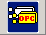
\includegraphics[scale=1]{Img/logo/logo_OPClient.PNG} 
\end{wrapfigure}

\textbf{ }\\
- le logiciel OPC Client (ApClient.exe) qui permettait de communiquer directement avec les automates disponibles via une interface graphique.

\begin{wrapfigure}{r}{0.1\textwidth}
	
\includegraphics[scale=1]{Img/logo/logo_PCNetInt.PNG} 
\end{wrapfigure}

\textbf{ }\\
- et le logiciel PC Networking Interface (console.exe) pour voir comment étaient paramétrés certains automates et sur quel serveur étaient-ils raccordés.\\

Pour réaliser des tests au fur et à mesure du développement, j’ai travaillé en local (sur le serveur qui héberge le serveur OPC (90)) avec les variables nommées DB1 du logiciel Applicom (variables locales). Ainsi, la connexion était toujours accessible sur le serveur ce qui m’a permis de tester et de déboguer ApplicomDB1. L'application était plutôt basique puisqu’elle donnait à l’utilisateur l’accès à quatre boutons (Connexion, Déconnexion, Envoi et Lecture) et à deux champs de texte (un pour pouvoir envoyer une donnée vers l’automate et l’autre utilisé pour afficher la valeur lue).\\

\centerline{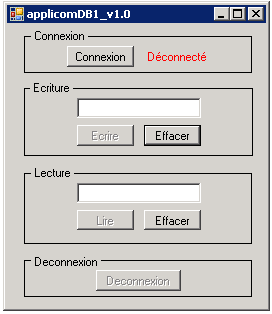
\includegraphics[scale=1]{Img/Capture_applicomDB1v1.PNG}}
\centerline{\textbf{\underline{Capture de l’application applicomDB1.}}}
\espace{}

À la suite de cette première version, j’en ai développé une deuxième en utilisant la bibliothèque graphique XAML\textcolor{red}{*} qui était utilisée sur MesToColis. Celle-ci ne changeait rien aux fonctionnalités de l’application mais me familiarisait un peu plus avec l’environnement de développement à modifier. Une fois le développement terminé, j’ai pris un peu de temps pour étudier de plus près le code des fonctions qui composent MesToColis.\\
\alinea
	De cette analyse, j’ai dressé un bilan de toutes les modifications nécessaires pour le nouveau fonctionnement de l’application à la suite de quoi j’ai réalisé les premiers diagrammes de séquence UML\textcolor{red}{*} (de l'envoi de données) et le nouveau schéma fonctionnel\textcolor{red}{*} (voir annexes \emph{Diagramme de séquence} et \emph{Schéma fonctionnel}).\\
Une fois l’analyse terminée et les modifications à réaliser validées par M. Deschamps Stéphane, j’ai commencé à travailler sur le développement de MesToColis.
	
	\subsection{Développement de MesToColis}
	\subsubsection{Introduction}
		\paragraph{}
	
	Dans un souci d’organisation, M. Deschamps et moi-même avons divisé le déroulement du projet en différentes périodes. À la base, le développement de MesToColis devait être fait sur deux mois, suite à quoi une autre période de deux mois était destiné à l’optimisation de l’application (comme spécifié sur le cahier des charges).\\
En revanche, cette organisation a été revue au cours du stage puisqu’une autre période a vu le jour.\\
En effet, une période d’évolution d’affichage des OFs a été ajouté entre la phase de développement et la phase d’optimisation. C’est pourquoi les trois prochaines sous-parties expliciteront les actions réalisées durant ces différentes périodes.
	
	\subsubsection{Modification de l’application MesToColis}
		\paragraph{}
	
	Alors que je venais de terminer le développement d’applicomDB1 et l’analyse de pré-développement de MesToColis, j’ai commencé à modifier l’application. J’ai donc commencé avec la dernière version de MesToColis qui était disponible à ce jour. Celle-ci était destinée à un autre site de production et avait été développée par M. Réau Pierrick. L’une des premières choses à revoir a donc été de mettre à niveau l’application pour qu’elle soit adaptée au fonctionnement du site de production de TLM. J’ai donc ajouté quelques paramètres, notamment “RechercheMasque” (à OUI ou NON).
En effet, sur la version existante de MesToColis, l’application faisait une vérification entre le code de la machine passé en paramètre et l’id du masque au sein d’une base de données (ces deux paramètres devaient être liés). Sur le site de TLM, aucun lien comme celui-ci n'était pas fait puisqu’un seul format de masque est utilisé. Donc, ce nouveau paramètre permettait d’éviter cette recherche de masque. En contrepartie, il a fallu ré-utiliser deux autres paramètres qui étaient déjà en place sur l’application : “Masque” et “PathMasque”. Ceux-là désignent respectivement le nom du masque qu’on souhaite charger et le chemin vers le dossier qui le contient.\\
\alinea
Une fois cette mise à niveau réalisée, j’ai dû ensuite retravailler le format du masque de TLM puisque la lecture de celui utilisé par le logiciel iDaro n’était pas géré par la version de l’application. J’ai donc choisi de modifier le masque pour qu’il puisse être directement lu avec la fonction existante (pour le site MTT). On retrouve alors ce format de masque : \\

\centerline{\includegraphics[scale=0.9]{Img/Img_MasqueVIDEOJETDirect.PNG}}
\centerline{\textbf{\underline{Masque provisoire de TLM (format type MTT).}}}
\espace{}

Cette modification ne venait pas perturber le temps de développement qu’on avait prévu à la base puisque suite à cette période sur deux mois, une phase d’optimisation de l’application était prévue dans laquelle je devais modifier la lecture et le format du masque de TLM pour qu’il puisse être lu au format XML. Une fois la lecture du masque de TLM gérée, j’ai constaté qu’il y avait quelques problèmes dans la lecture des données pour un OF sélectionné ou une UT rentrée. Pour trouver d’où provenait l’erreur, M. Deschamps Stéphane a su m’aider pour comprendre comment les requêtes SQL\textcolor{red}{*} était faites et d’où l’erreur pouvait provenir. Une fois les modifications sur ces requêtes réalisées, l’ensemble des informations qui composent le masque et leurs valeurs pour un OF ou une UT saisie étaient bien lues.

	\subsubsection{Tests d'étiquetage avec MesToColis}
		\paragraph{}
	
	Une fois le code fonctionnel, M. Marais Sébastien m’a mis à disposition un automate avec une documentation sur les différents espaces mémoire à viser afin de pousser un peu plus loin les tests. J’ai donc eu l’occasion de paramétrer l’automate pour le rendre accessible sur le serveur OPC via le logiciel PC Network Interface. Une fois bien installé, j’ai dû revoir la fonction d’envoi de données puisque les mots de l’automate n’étaient pas paramétrés comme je le pensais.\\
En effet, il fallait prévoir deux types d’envoi puisque certaines informations d’étiquetage (ex : libellé du produit, lot UVC... etc) devaient être comprises sur un intervalle de mots de l’automate alors que d’autres étaient compris sur un seul mot. Cette différence était liée au fait que les mots des automates pouvaient être signés ou non, ainsi la valeur d’un mot signé était comprise entre -32768 et +32767.

\begin{center}
	\begin{tabular}{|l|c|}
	\hline
		Type de variable & Valeurs possibles de la variable \\
	\hline
		VT\_UI1 & from 0 to 255 \\
		VT\_I1 & from -128 to 127 \\
		VT\_UI2 & from 0 to 65535 \\
		VT\_I2 & from -32768 to 32767 \\
		VT\_UI4 & from 0 to 4294967295 \\
		VT\_I4 & from -2147483648 to 2147483647 \\
		VT\_R4 & from -3.4e+38 to 3.4e+38 \\
		VT\_R8 & from -1.79e+308 to 1.79e+308 \\
	\hline
	\end{tabular}
\end{center}

Dans le cadre de l’envoi de données de MesToColis vers l’automate, on avait alors deux nouvelles fonctions d’envoi : \\

\begin{enumerate}[•]
	\item EnvoiCar qui avait comme paramètre une valeur à envoyer et un intervalle de mot de l’automate. Celle-ci envoyait chaque caractère compris dans la valeur à envoyer vers la plage de mot de l’automate.
	\item EnvoiVal qui avait pour paramètre une valeur à envoyer et un seul mot de l’automate. Celle-ci envoyait directement la valeur vers le mot de l’automate.
\end{enumerate}

\centerline{\includegraphics[scale=0.6]{Img/Img_SchemaAutomate.PNG}}
\centerline{\textbf{\underline{Schématisation des différentes fonctions d'envoi.}}}
\espace{}

Après ces modifications prisent en compte, les phases de tests ont pu commencer en vérifiant que la fonction d’envoi des données était bien fonctionnelle et que les valeurs envoyées à l’automate étaient les mêmes affichées sur l’écran tactile fourni avec.\\

\centerline{\includegraphics[scale=0.6]{Img/Capture_AffichageAutomate.PNG}}
\centerline{\textbf{\underline{Résultats des tests d'envoi de données.}}}
\espace{}

Une fois les tests réalisés et concluants, j’ai passé un peu de temps à faire les quelques modifications demandées par M. Deschamps Stéphane. Ayant terminé le développement du nouveau mode de fonctionnement de l’application, je suis passé en phase d’évolution de l’affichage des OFs.

	\subsubsection{Evolution d’affichage de l’application}
		\paragraph{}
	
	Cette phase d’évolution a été assez courte et est apparue juste avant celle de l’optimisation. Celle-ci concernait l’affichage des OFs de MesToColis et était traduite par la modification des requêtes SQL pour aller chercher les OFs selon plusieurs codes machine ou plusieurs compétences, plusieurs modifications étaient donc à prévoir.\\
La première d'entre elles a été la modification du type de paramètre lors du lancement de l’application. En effet, le premier d’entre eux est le code machine et celui-ci devait désormais être un code machine (ou plusieurs séparés par un pipe “|”) ou une compétence (ou plusieurs séparées par un pipe).\\
Une compétence, sur TLM, est attribuée à une ligne de production, par exemple la ligne 98 de TLM est une ligne de suremballage, elle possède donc la compétence “Suremballer”.\\
Il a donc fallu réaliser beaucoup de changements au sein du code notamment lors du lancement de MesToColis puisque auparavant, un objet de type machine était créé en fonction du code machine passé en paramètre. Avec ce nouveau fonctionnement il a fallu changer la création d’un objet machine en une liste d’objet machine.\\

\centerline{\includegraphics[scale=1]{Img/Img_EvolutionMES1.PNG}}
\centerline{\textbf{\underline{Schématisation de la création d’une liste (ou d’un objet) de machine.}}}
\espace{}

Suite à cette modification, il a fallu aussi faire le lien entre une compétence et un code machine pour qu’une liste d’objets machine (ou un seul) puisse être créée lorsqu’une compétence (ou plusieurs) était passée en paramètre de l’application.\\

\centerline{\includegraphics[scale=1]{Img/Img_EvolutionMES2.PNG}}
\centerline{\textbf{\underline{Schématisation de la création d’une liste de machine en fonction d’une ou plusieurs compétence.}}}
\espace{}

Malheureusement, ces modifications n’ont pas été concluantes puisque cela rendait l’affichage des OFs ainsi que le fonctionnement de l’application trop compliqué à gérer avec le paramétrage existant (surtout pour les utilisateurs). Je suis donc reparti avec la version de MesToColis fonctionnelle pour passer en phase d’optimisation.
	
	\subsubsection{Optimisation de l’application}
		\paragraph{}
	
	Dans la phase d’optimisation, deux modifications majeures étaient à réaliser. En effet, la première optimisation concernait le format du masque de TLM ainsi que sa lecture et l’autre était d'ajouter un paramétrage par machine au sein de l'application (le code machine étant la clé).\\
J’ai d’abord travaillé sur le nouveau format du masque afin de le rendre plus homogène. En m’inspirant de celui qui était utilisé par le logiciel iDaro, j’ai su en créer un autre et le faire valider par M. Deschamps Stéphane(voir annexe Masque XML de TLM).\\
J’ai ensuite modifié la fonction de lecture du masque et d’écriture du fichier tmp lorsque MesToColis est lancé en mode SERVICE. Dans un souci d’uniformisation, j’ai tenu à garder la fonction qui gérait le chargement, l’écriture et la lecture des masques pour le site de MTT pour qu’à l’avenir, une seule et même version de l’application soit installée sur différents sites de production (MTT et TLM par exemple). J’ai donc ajouté une vérification à la lecture des premières lignes du fichier pour qu’il remarque s’il s’agissait bien du nouveau format de masque ou non.\\
La vérification faite, j’ai développé la fonction pour que toutes les balises qui composent le masque soient bien lues et remplacées (dans le cas d’un fonctionnement en mode SERVICE).\\
Suite à cette modification, j’ai commencé à travailler sur la deuxième optimisation. Celle-ci avait pour but de modifier le paramétrage pour que l'application soit paramétrable avec une machine donnée. Ainsi, lors du déploiement sur le site de production, qu’on se retrouve sur une machine de la ligne 98 ou bien de la ligne 99, chacune d’elles retrouverait son propre paramétrage.\\
J’ai donc passé un peu de temps avec M. Réau Pierrick pour voir quelle serait la nouvelle forme de paramétrage la plus adéquate. Suite à cette entrevue, j’ai proposé le nouveau modèle à M. Deschamps Stéphane pour qu’il le valide.\\
J’ai commencé par revoir le fichier de paramétrage de base de l’application pour mettre en commentaires les paramètres qui seraient propres à une machine. Ensuite, j’ai créé un nouveau groupe de paramètres nommé “paramMachine” pour les stocker. Je n’ai pas rencontré de soucis techniques pour le faire mais j’ai eu besoin d'une réunion avec M. Réau Pierrick au cours du développement ce qui m’a permis d’observer un problème de conception du nouveau groupe de paramètre.\\

Une fois la mise en place de ces deux optimisations, j’ai pu réaliser les derniers tests d’étiquetage en présence de M. Marais Sébastien avec l’étiqueteuse Mulet. Ceux-là se sont avérés concluants puisque pour n’importe quel code machine lancé en paramètre le chargement, l’envoi et l’étiquetage des données étaient corrects. Les tests étant validés, une mise en production a pu être proposée pour la semaine 27.\\
	
	\clearpage
	
	\section{Problèmes rencontrés}
		\paragraph{}
	
	Les problèmes que j’ai pu rencontrer sont plutôt nombreux et sont tous synthétisés sur le GIT du stage dans le fichier ProblemesRencontres.txt. Vous retrouverez sur ce fichier l’ensemble des difficultés et problèmes rencontrés ainsi que les hypothèses, essais et solutions trouvés pour chacun d’entre eux.\\
Dans cette partie, je ne présenterais que ceux qui m’ont causé le plus de difficulté à résoudre.
Au-delà des petites difficultés rencontrées comme des erreurs d’instanciation (initialisation d’un objet), de déclaration d’objet, de syntaxe ou des problèmes avec l’environnement de développement (etc), j’ai rencontré différents types de problèmes regroupés dans les catégories suivantes : communication, conception, développement et système.\\

\textbf{COMMUNICATION}\\
\\
\emph{Problème :} \textbf{L’automate de test sur TLM était injoignable.}\\
\\
\emph{Hypothèses :}

\begin{enumerate}[-]
    \item La prise Ethernet sur laquelle est branché l’automate n’est pas brassée ? Si pourtant.
    \item Le problème provient peut-être du Firewall ? Non, il est désactivé.
    \item Le port d’émission de l’automate visé n’est pas le bon ? Non spécifié sur les autres communications avec le même automate.
\end{enumerate}

\emph{Tests :}

\begin{enumerate}[-]
    \item Mise sur réseau Ethernet et tentative de ping : le ping renvoie bien les octets.
    \item Modification de la passerelle de l’automate : même résultat.
\end{enumerate}

\emph{Solution :} Mise en service de l’automate sur réseau OPC Applicom.ServeurOPC.1 via le logiciel PC Network Interface.\\

\textbf{CONCEPTION}\\
\\
\emph{Problème :} \textbf{Le lot UVC n’est pas chargé.}\\
\\
\emph{Hypothèses :}

\begin{enumerate}[-]
    \item Le programme ne rentre pas dans la fonction dynamique pour le lot UVC, est-ce normal ? Oui, car le paramètre ID\_Machine n’est pas géré sur le site de production TLM.
    \item Le lot UVC doit-il toujours être lu ? Non, seulement en mode UT. En mode OF, il est entré par l'utilisateur.
\end{enumerate}

\emph{Tests :}

\begin{enumerate}[-]
    \item Test en mode OF : l'information est manquante.
    \item Test en mode UT (022104170158003) avec une version antérieure de MesToColis sur TLM : il est bien chargé.
    \item Prise d’informations avec M. Ribreau Fabien : ce n’est pas un problème, l’utilisateur doit le rentrer.
\end{enumerate}

\emph{Solution :} La fonction dynamique pour le lot UVC n’est pas fonctionnelle (ID\_Machine non géré sur TLM) donc le lot UVC est à rentrer directement par l’utilisateur.
\begin{center}
	\rule{8cm}{0.1pt}
\end{center}

\emph{Problème :} \textbf{Le nouveau paramétrage machine de l’application lève des exceptions.}\\
\\
\emph{Hypothèses :}

\begin{enumerate}[-]
    \item Une balise regroupant plusieurs éléments est-elle nécessaire ? Peut-être.
    \item La fonction de lecture des arguments est-elle correctement placée ? Oui.
\end{enumerate}

\emph{Tests :}

\begin{enumerate}[-]
    \item Ajout d'un groupCollection pour ajouter une balise <Groupe machine=""> : une erreur ressort tout le temps ("ID" non reconnu).
    \item Copie d'une même ligne pour qu'il y ait deux balises <group ID="" adresse=""> : la même erreur ressort.
    \item Copie sur brouillon des différents types de balise pour le fichier des étiqueteuses et celui des automates : erreur de conception entre groupCollection et groupElement.
    \item Rendez-vous avec M. Réau Pierrick : restructuration de la conception du paramétrage.
\end{enumerate}

\emph{Solution :} Le problème provenait de ma conception. En effet, dans un fichier de paramétrage il est obligatoire qu’une collection enveloppe des éléments.\\

\textbf{DÉVELOPPEMENT}\\
\\
\emph{Problème :} \textbf{Le numéro d’OF n'apparaît pas.}\\
\\
\emph{Hypothèses :}

\begin{enumerate}[-]
    \item Le numéro d’OF est-il toujours accessible ? Non, seulement en mode OF.
    \item Les paramètres passés dans les requêtes SQL doivent être différents selon le mode de fonctionnement de l’application ? Oui, mode UT c’est l’UT saisie qui est pris comme paramètre alors qu’en mode OF c’est le résultat d’une requête SQL qui est pris.
\end{enumerate}

\emph{Tests :}

\begin{enumerate}[-]
    \item Débogage de l’application pour vérifier quelles informations sont passées en paramètre pour la requête SQL : la valeur passée en paramètre n’est pas la bonne pour le mode OF.
\end{enumerate}

\emph{Solution :} La requête SQL attendait un numéro d’OF alors qu’elle recevait un numéro d’UT entré en mode UT.
\begin{center}
	\rule{8cm}{0.1pt}
\end{center}

\emph{Problème :} \textbf{Le nombre d’OF affiché est beaucoup trop grand avec les compétences en paramètre.}\\
\\

\emph{Hypothèses :}

\begin{enumerate}[-]
    \item Une modification serait à apporter à la requête SQL ? Surement (un DISTINCT ?).
\end{enumerate}

\emph{Tests :}

\begin{enumerate}[-]
    \item Tests sur la base de données avec Oracle SQL Developer avec M. Deschamps Stéphane : le souci provient de ma requête SQL.
\end{enumerate}

\emph{Solution :} La liaison entre le code machine et une compétence n’était pas faite mais le nombre d’OF affiché est encore trop grand (souci de l’évolution).\\

\textbf{SYSTEME}\\
\\
\emph{Problème :} \textbf{L’envoi de données vers l’automate n’est pas affiché (valeur reste à zéro).}\\
\\
\emph{Hypothèses :}

\begin{enumerate}[-]
    \item Les valeurs envoyées sont trop grandes ? Peut-être.
	\item Les mots des automates sont peut-être signés ? Surement.
\end{enumerate}

\emph{Tests :}

\begin{enumerate}[-]
    \item Envoi de données avec le logiciel OPClient : la valeur s’affiche.
	\item Test avec des valeurs plus ou moins grandes : le maximum est atteint à 32467.
\end{enumerate}

\emph{Solution :} Le mot de l’automate était signé (+ ou -34567), modification de celui-ci en non signé.
\begin{center}
	\rule{8cm}{0.1pt}
\end{center}

\emph{Problème :} \textbf{L’application crash dès le lancement de celle-ci.}\\
\\
\emph{Hypothèses :}

\begin{enumerate}[-]
    \item Une modification apportée au programme ne convient pas ? Non, les modifications ont été faites uniquement dans le cas où l'automate n'est pas joignable (gestion d’erreur).
	\item Le problème est causé par la compilation de la solution de l’application ? Oui, l'erreur affiche une modification du fichier Application.g.vb.
	\item Y a-t-il un problème de lien entre les fichiers ? Je ne pense pas.
\end{enumerate}

\emph{Tests :}

\begin{enumerate}[-]
    \item Multiple test sans résultat : il y aurait eu une modification sur le fichier application.g.vb.
	\item Un message s’affiche : “Le fichier Application.g.vb a été modifié de l'extérieur, chargement de celui-ci ? Oui/Non” : Quelle que soit la réponse, rien ne change.
	\item Régénération de la solution : le problème est résolu.
\end{enumerate}

\emph{Solution :} Problème encore inconnu (bug de Visual Studio ?).
\begin{center}
	\rule{8cm}{0.1pt}
\end{center}

\emph{Problème :}\textbf{Le lancement de l’application sur le serveur de production (et de test) génère une exception liée aux paramètres COM/DCOM.}\\
\\
\emph{Hypothèses :}

\begin{enumerate}[-]
    \item Le fichier OPCDAAuto.dll est peut-être défectueux ? Pas impossible mais très douteux puisque l'installation a correctement copié les autres fichiers dlls (ex : log4net.dll). De plus, celui-ci fonctionnait correctement avant l'installation.
	\item La connexion n'est pas autorisée à cause de l’accès NAC et de l'ouverture des ports des automates qui n’a pas été réalisé ? Probable mais déjà demandé auprès de M. Mauny Gaetan.
	\item Le système (du serveur) ne reconnaît pas le nouveau fichier dll utilisé pour la connexion vers un automate (OPCDAAuto.dll) ? Très peu probable puisque c'est la même chose qu'avec le fichier log4net qui est actuellement utilisé (RegSvr32).
	\item Un service serait manquant ? OPCEnum.exe apparaît sur le serveur 94 mais pas sur le serveur TSE 04.
	\item Le service OPCEnum n'est plus d'actualité (obsolète) et doit être remis à jour ? Peut-être.
	\item Les droits d'accès ne nous sont pas donnés avec la configuration COM/DCOM ? Non puisque la configuration est correcte, vérifiée avec les fichiers cmopmgmt.msc et comexp.msc.
	\item Paramètres manquants pour la fonction connect ? Oui par la suite, il manquait un objet string contenant l'adresse IP du serveur sur lequel on souhaite se connecter.
\end{enumerate}

\emph{Tests :}

\begin{enumerate}[-]
	\item Schématisation du problème.
	\item Essai de connexion au serveur OPC avec comme paramètre le CLSID du serveur : toujours la même erreur.
	\item Utilisation d'un petit applicatif nommé MyOPCClient afin de voir quels sont les serveurs que l'on peut trouver : problème avec certains serveurs (freeze, délai trop long ou connexion impossible).
	\item Prise de contact avec M. Mauny Gaetan afin de demander les accès NAC et l'ouverture des ports pour les automates du serveur de test et de production : les accès sont déjà donnés.
	\item Modification de la configuration COM/DCOM des serveurs 90 et 94 (test) et des TSEs 02 et 04 (production) : toujours impossible de communiquer avec l'automate.
	\item Modification des propriétés du bouton dans la VTR : réception d’un mail avec la même erreur.
	\item Utilisation de la commande RegSvr32 afin de "sauvegarder" la dll OPCDAAuto sur le système : sauvegarde réussie mais ne change rien, l'erreur est toujours là même.
	\item Mise à jour du service OPCEnum pour la dernière version (juin 2016) : toujours le même problème.
	\item Prise de contact par mail avec M. Randy Kondor de la OPCFoundation (États-Unis): conseil d'utilisation de l'outil OPCExpert afin d'analyser les problèmes de connexion.
	\item Utilisation de l'outil OPCExpert : le logiciel signale un problème sur le serveur de test de TLM avec la connexion au serveur applicom du 94, le service OPCEnum est défaillant.
	\item Utilisation de la solution donnée par OPCExpert : la connexion est disponible, envoi de données vers l'automate réussi (avec la modification de la fonction connect) mais il faut qu’OPCExpert soit toujours installé.
	\item En cochant "Tools/Options/Enable essentials OPC features" l'application se lance : dans un dossier, la seule différence avec cette action est l'apparition de certaines DLLs, le problème viendrait donc de certaines dlls manquantes ? Peut-être.
	\item Mise en place du dossier OPCExpert avec le fichier d'installation OPCExpert.rar et du dossier contenant les DLLs générées : l’application se lance bien et se connecte bien à l’automate.
\end{enumerate}

\emph{Solution :} Le problème provenait de deux choses : 

\begin{enumerate}[-]
	\item D'abord la fonction connect devait recevoir en plus du nom du serveur OPC, l'adresse IP du PC qui l'héberge.
	\item Enfin, le service OPCEnum devait être revu sur chaque poste client OPC via le logiciel OPCExpert afin de pouvoir accéder aux automates.
\end{enumerate}
	
	\clearpage
	
	\section{État final du projet}
		
	\subsection{Présentation du projet final}
		\paragraph{}
	
	Aujourd’hui, la nouvelle version de l’application MesToColis (1.1.17292.0) est installée sur les serveurs TSE 02, 03, 06 et 07 du site de production de TLM et gère la connexion OPC entre le logiciel Mes et l’automate\\
API\_DEPOSE\_ETIQ\_L99\_TLM disponible sur le serveur distant TSE 04. L’utilisateur en production a accès à deux nouveaux boutons, un pour observer la quantité d'encre et d’étiquette de l’étiqueteuse Mulet et un pour lancer l’application MesToColis vers le Mulet. En la lançant, il lui suffit de flasher un code d’une UT pour que le chargement des données se fasse. Une fois les valeurs chargées, l’utilisateur est amené à les envoyer pour que l’automate les relance vers l’étiqueteuse.\\
Enfin, pour sortir l’étiquette, la personne doit appuyer sur le bouton d’impression de l’afficheur tactile de l’étiqueteuse.\\
Cette installation a été réalisée pour utiliser le Mulet en attente d’un arrêt usine pour tester le système avec les deux étiqueteuses du portique Jyga de la production des lignes 98 et 99.
	
	\subsection{Améliorations possibles}
		\paragraph{}
	
	Même si le système installé est fonctionnel, il reste néanmoins quelques améliorations possibles. En effet, la première d’entre elles serait de pouvoir ajouter un champ pour qu’on y informe combien d’étiquette l’utilisateur souhaite sortir. Cependant, cette amélioration semble plus compliquée que prévu puisque l’étiquette reste collée au support en attendant d’être prise par l'utilisateur.\\
La deuxième amélioration serait d’attendre de recevoir un message de l’automate pour qu’un panel de valeurs test soit envoyé, ainsi un éventuel problème de communication serait directement identifié. Cependant, cette amélioration reste en standby puisque l’utilisateur ne se sert pas uniquement de MesToColis et nécessiterait à l’application d’attendre un message de l’automate.\\
Enfin, la dernière amélioration serait d’installer la même version de l’application sur l’ensemble des sites de production qui utilisent MesToColis (c’est-à-dire MTT, Cambrais et TLM) avec pour seule différence, le fichier de configuration de l’application.\\
		
	\clearpage
	
	\section{Conclusion}
		\paragraph{}
			
	Ce projet m’a été proposé par M. Deschamps Stéphane lors de la période de stage en entreprise du 03 avril 2017 au 31 juillet 2017. Durant ce stage, j’ai dû réaliser une modification sur l’application d’étiquetage de colis MesToColis associé au projet “Suppression du logiciel iDaro”.\\
Aujourd’hui, je pense répondre aux attentes finales du projet c’est-à-dire de pouvoir réétiqueter une étiquette via l’étiqueteuse Mulet avec le protocole de communication avec un automate (OPC). En effet, j’ai réussi à redévelopper en interne (à l’entreprise) cette communication entre le logiciel MES et l’automate qui était auparavant sous-traité par une entreprise. Cette même solution sera surement utilisée dans les mois à venir pour gérer l’intégralité de la communication avec les étiqueteuses des lignes de productions 98 et 99.\\
Il reste néanmoins quelques modifications possibles pour compléter la réalisation. Tout d’abord, il serait possible de reprendre l’évolution de l’affichage des OFs en fonction d’un ou plusieurs codes machine mais aussi en fonction d’une ou plusieurs compétences. Aussi, il serait possible de revoir le test de connexion pour qu’à la réception d’un message de l’automate, le logiciel MES puisse envoyer un panel de valeurs test.\\
À l’issue de ce projet, j’ai pu travailler en complète autonomie sur le site de Chantonnay (TLM) mais aussi en équipe sur les différents sites de production avec Marais Sébastien, Guilloteau Kévin , Deschamps Stéphane, Réau Pierrick et Ribreau Fabien.\\
J’ai su m'immiscer dans la vie d’un développeur informatique et observer quels objectifs, attentes et obligations que ce métier pourrait exiger. La conception du cahier des charges, le développement, l’installation, l’assistance ainsi que la rédaction de documentation (spécification détaillée et procédure d’utilisation) sont des étapes clés du métier d’analyste programmeur. Je ressors donc de ce stage avec un avant-goût du métier que j’aimerais faire.\\
De plus, mettre à profit ses connaissances pour faciliter le travail d’autres personnes m’a poussé à fournir au final un système qui répond aux conditions et aux attentes des utilisateurs. Ce stage a donc été intéressant puisque la production sortante de celui-ci a pu être testée et observée directement sur le site de production, ce qui m’a donc motivé à rendre ce projet fonctionnel à temps.\\
Enfin, je tiens à exprimer mon entière satisfaction d’avoir pu travailler dans de bonnes conditions matérielles et dans un environnement agréable tout le long de la période du stage.\\

	\clearpage

	\section{Sources}
	
	Lien vers le GIT : \\
\url{https://github.com/qfresneau/Stage}\\

	Autres liens utiles : \\ 
\url{https://opcfoundation.org/}\\
\url{https://www.w3schools.com/sql/}\\
\url{https://social.msdn.microsoft.com/Forums/fr-FR/home}\\
\url{https://www.automation.com/pdf_articles/Troubleshooting_OPC_and_DCOM.pdf}\\
	
	\section{Glossaire}
	
GMS : Grandes et Moyennes Surfaces.
MES : Un Manufacturing Execution System (MES) (traduit en français par : gestion des processus industriels) est un système informatique dont les objectifs sont d'abord de collecter en temps réel les données de production ce qui permet ensuite de réaliser un certain nombre d'activités d'analyse (traçabilité, contrôle de la qualité, suivi de production, ordonnancement, maintenance...).\\
TLM : (Traiteur de La Mer) Il s'agit des initiales du nom d'un des sites de production de Chantonnay.\\
MTT : (Montifaut Traiteur) Il s'agit des initiales du nom d'un des sites de production de Montifaut.\\
OF : Sur le site de TLM, un OF correspond à un ordre de fabrication d'un produit.\\
UT : Sur le site de TLM, une UT est une unité de traçabilité (une UT est liée à un OF).\\
VB.net : Visual Basic .NET est la nouvelle génération du langage Visual Basic. Il représente un moyen simple et rapide de créer des applications .NET, y compris des services Web XML et des applications Web.\\
UML : Le langage de modélisation unifié (Unified Modeling Language), est un langage de modélisation graphique à base de pictogrammes conçu pour fournir une méthode normalisée pour visualiser la conception d'un système.\\
XML : L'eXtensible Markup Language est un langage informatique balisé.\\
OPC : Se traduit par OLE (Object Linking and Embedding) for Process Control. OPC est un protocole de communication mais aussi une technique basée sur les techniques OLE, COM, et DCOM développées par Microsoft pour sa famille de systèmes d'exploitation Windows.\\
SQL : SQL (Sructured Querry Language) est un langage informatique normalisé servant à exploiter des bases de données relationnelles.\\
XAML : Le langage XAML (Extensible Application Markup Language) est un langage de balisage basé sur XML développé par Microsoft. XAML est le langage qui se trouve derrière la présentation visuelle des applications que vous développez dans Microsoft Expression Blend, tout comme HTML constitue le langage à la base de la présentation visuelle d’une page Web.\\
	
	\clearpage
	
	\section{Annexes}
	
		\begin{center}
	\centerline{\includegraphics[scale=0.7,angle=270]{Img/OrganisationDSI.PNG}}
	\espace{}
	\centerline{\textbf{\underline{Organisation de la DSI.}}}
		\end{center}
	
	\clearpage
	
		\begin{center}
	\centerline{\includegraphics[scale=0.65,angle=270]{Img/ArchitectureMES.PNG}}
	\espace{}
	\centerline{\textbf{\underline{Architecture des serveurs MES.}}}
		\end{center}
	
	\clearpage
	
		\begin{center}
	\centerline{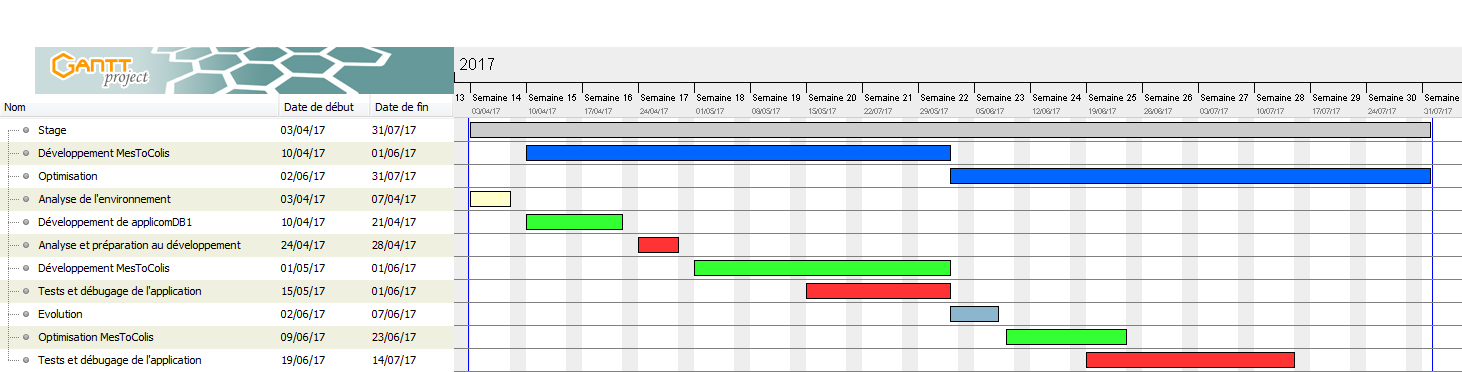
\includegraphics[scale=0.5,angle=270]{DiagrammeDeGantt}}
	\espace{}
	\centerline{\textbf{\underline{Diagramme de Gantt.}}}
		\end{center}
	
	\clearpage
	
		\begin{center}
	\centerline{\includegraphics[scale=0.23]{Img/Img_DSEnvoiAuto2.PNG}}
	\espace{}
	\centerline{\textbf{\underline{Diagramme de séquence lors de l'envoi de données.}}}
		\end{center}
		
	\clearpage
	
		\begin{center}
	\centerline{\includegraphics[scale=0.24]{Img/Img_SFDapres.PNG}}
	\espace{}
	\centerline{\textbf{\underline{Nouveau schéma fonctionnel de l'application.}}}
		\end{center}
	
	\clearpage
	
		\begin{center}
			\lstinputlisting{Img/tlm2.xml}
			\centerline{\textbf{\underline{Nouveau masque XML de TLM.}}}
		\end{center}
	
	\clearpage
	
\end{document}
\newline